\documentclass[10pt,a4paper]{article}
\usepackage{ngerman}
\usepackage[utf8]{inputenc}
\usepackage{sectsty, xcolor}
\usepackage{lastpage}
\usepackage{amsmath, amsfonts, amssymb, enumitem, fancyhdr, graphicx, float, makeidx, textcomp, multicol}
\usepackage[hidelinks]{hyperref}
\usepackage[hang,flushmargin]{footmisc}
\usepackage{listings}
\lstloadlanguages{HTML}
\definecolor{pblue}{rgb}{0.13,0.13,1}
\definecolor{pgreen}{rgb}{0,0.5,0}
\definecolor{pred}{rgb}{0.9,0,0}
\definecolor{pgrey}{rgb}{0.46,0.45,0.48}
\definecolor{background}{rgb}{0.95,0.95,0.92}
\lstset{language=HTML,
  backgroundcolor=\color{background},
  frame=single,
  rulecolor=\color{pgrey},
  showspaces=false,
  showtabs=false,
  breaklines=true,
  showstringspaces=false,
  breakatwhitespace=true,
  commentstyle=\color{pgreen},
  keywordstyle=\color{pblue},
  stringstyle=\color{pred},
  breaklines=true,
  numbers=left,
  numberstyle=\tiny\color{pgrey},
  basicstyle=\ttfamily\footnotesize,
  inputencoding=utf8,
  extendedchars=true,
  literate={ä}{{\"a}}1 {ö}{{\"o}}1 {ü}{{\"u}}1,
  moredelim=[il][\textcolor{pgrey}]{\$\$},
  moredelim=[is][\textcolor{pgrey}]{\%\%}{\%\%}
}
\makeindex

\definecolor{dunkelblau}{rgb}{0,0.4,0.6}
\subsectionfont{\color{dunkelblau}}

\title{WEBT FS 2020}
\author{Victor Fernández}
\date{Februar 2020}

\addtolength{\oddsidemargin}{-.875in}
\addtolength{\evensidemargin}{-.875in}
\addtolength{\textwidth}{1.75in}
\addtolength{\topmargin}{-.875in}
\addtolength{\textheight}{1.75in}

% muss nach Änderung der margin kommen!
\pagestyle{fancy}
\fancyhf{} %reset
\fancyhead[L]{HSLU}
\fancyhead[C]{WEBT}
\fancyhead[R]{\thepage/\pageref{LastPage}}
\fancyfoot[L]{}
\fancyfoot[C]{}
\fancyfoot[R]{}
\renewcommand{\headrulewidth}{0.2pt} % Strich in Kopfzeile

\begin{document}

\maketitle
\tableofcontents
\thispagestyle{empty}
\pagebreak

\section{SW01 - Funktionen}
\begin{tabularx}{\textwidth}{|rX|}
    \hline
        \textbf{\textcolor{blue}{Thema:}}&Grundlegendes zu reelwertigen Funktionen\\
        \textbf{\textcolor{blue}{Ziele:}}&\vspace{-4mm}\begin{itemize}
            \item Sie kennen die Grundbegriffe im Zusammenhang mit Funktionen (wie Funktionsvorschrift, Wertetabelle, Graph, Definitions- und Wertebereich, etc.).
            \item Sie kennen die Familie von linearen, Exponential- und Logarithmusfunktionen, den Differenzenquotienten und können Graphen von Funktionen qualitativ beurteilen (z.B. Parameter ablesen, etc.).
            \item Sie können den Graphen einer Funktion verschieben und skalieren und überprüfen ob die Funktion gerade oder ungerade ist.
            \item Sie können die Umkehrfunktion bestimmen
        \end{itemize}\\
        \textbf{\textcolor{blue}{Resultate:}}&Sie können sicher mit Funktionen, insbesondere linearen und Exponentialfunktionen umgehen.\\
        \textbf{\textcolor{blue}{Vorgehen:}}&Anhand vieler Beispiele sollen die wesentlichen Fälle, die in der Praxis vorkommen, studiert, analysiert und geübt werden.\\
    \hline
\end{tabularx}

\subsection{Funktionen und Änderungen}
\subsubsection{Begriffe}
\paragraph{Definition (Funktion (oder Abbildung))}
Eine \textbf{Funktion} ist eine Regel, die gewissen Objekten (hier Zahlen) als Inputs \textbf{genau ein} Objekt (hier eine Zahl) als eindeutigem Output zuordnet. Die Menge der Objekte aller Inputs heisst \textbf{Definitionsbereich} der Funktion, die Menge der resultierenden Outputs heisst \textbf{Wertebereich}. Der Input heisst unabhängige Variable, der Output abhängige Variable.
\paragraph{Bereiche}Für Funktionen verwendet man i.d.R. Buchstaben wie $f$, $g$, $h$, \dots, oder $F$, $G$, $H$, \dots Der \textbf{Definitionsbereich} der Funktion $f$ wird mit $D(f)$ bezeichnet, der \textbf{Wertebereich} mit $W(f)$. Als unabhängige Variable verwendet man normalerweise $x$, als abhängige Variable $y$.\\[1em]
$f: D(f)\rightarrow W(f),x\rightmapsto y=f(x)$\\[1em]

\todo{Diskrete vs stetige Grössen}
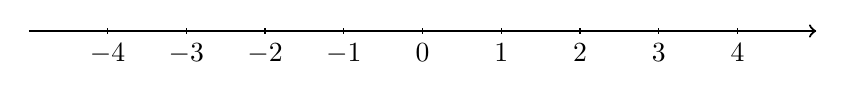
\begin{tikzpicture}
    \draw [->, thick] (-5,0) -- (5,0);
    \foreach \x in {-4,...,4}
        \draw (\x cm, 1pt) -- (\x cm, -1pt) node [anchor=north] {$\x$};
\end{tikzpicture}

\subsubsection{Darstellung}Darstellung von Funktionen mittels Wertetabellen, Graphen und Formeln (Funktionsvorschriften). Oder durch beschreiben, z.B.: \textsl{für jedes $x$ wächst $y$ um 1.5}.

\subsection{Einfache, lineare Funktionen}
\subsubsection{Monotonie}Funktionen können in einem \textbf{Abschnitt} (streng) monoton \textbf{steigend} oder (streng) monoton \textbf{fallend} sein. \\[1em]
\begin{tabularx}{\textwidth}{|rX|}
    \hline
    \textbf{Monoton steigend:}&Eine Funktion verläuft in einem Abschnitt teils horizontal, teils steigend.\\
    \textbf{Streng monoton steigend:}&Eine Funktion steigt in einem Abschnitt durchgehend, wird nie horizontal oder gar fallend.\\
    \textbf{Monoton fallend:}&Eine Funktion verläuft in einem Abschnitt teils horizontal, teils fallend.\\
    \textbf{Streng monoton fallend:}&Eine Funktion fällt in einem Abschnitt durchgehend, wird nie horizontal oder gar steigend.\\
    \hline
\end{tabularx}\\[1em]
Die Funktion kann (streng) monoton \textbf{steigend/fallend} sein, falls sie für alle x steigt oder fällt.

\subsubsection{Proportionalität}Wir sagen $y$ ist (direkt) proportional zu $x$, falls es eine Konstante $a$ gibt, sodass\\
$y=ax,\quad$ $a$ heisst \textsl{Proportionalitätskonstante}.

\subsubsection{Umgekehrt proportionale Funktionen}Beispiel: Die Durchschnittsgeschwindigkeit auf der Strecke $s=50km$ hängt umgekehrt proportional von der dafür benötigten Zeit $t$ ab, $v=\frac{s}{t}$. Heisst soviel, dass auch wenn sich die Strecke ändert, sich zwangsläufig auch die Zeit ändern muss, um die gleiche Durchschnittsgeschwindigkeit $v$ beizubehalten, z.B. $v=\frac{2\times 50km}{2\times t}$.

\subsubsection{Verschiebung und Skalierung von Funktionen}Verschiebt man eine Funktion $y=ax$ um $b$ in $y$-Richtung, erhält man die lineare Funktion $y=ax+b$.

\subsubsection{Differenzenquotient}Der \textbf{Differenzenquotient} von $f$ an der Stelle $x$ ist definiert durch:
\begin{align*}
    \frac{\Delta y}{\Delta x}=\frac{f(x+\Delta x)-f(x)}{\Delta x}
\end{align*}

\subsubsection{Gerade und ungerade Funktionen}
\begin{itemize}
    \item Eine gerade Funktion $f$ ist \textbf{achsensymmetrisch} bezüglich der $y$-Achse und es gilt:\\$f(-x)=f(x),\forall x \in D(f)$
    \item Eine ungerade Funktion $f$ ist \textbf{punktsymmetrisch} bezüglich dem Ursprung und es gilt:\\$f(-x)=-f(x),\forall x \in D(f)$
\end{itemize}
\subsection{Exponentialfunktionen}
\subsubsection{Begriffe}Eine Funktion der $f(x)=a\cdot b^x$ mit $b>0$ und $b\neq 1$ heisst \textbf{Exponentialfunktion}. $a$ heisst \textbf{Anfangswert} und $b$ heisst \textbf{Wachstumsfaktor}. Für Definitions- und Wertebereich gilt: $D(f)=\mathbb{R},\, W(f)=\mathbb{R^+}$


\subsection{Neue aus alten Funktionen}

\subsubsection{Verschiebung und Streckung}

\subsubsection{Zusammengesetzte Funktionen}

\subsection{Logarithmusfunktionen}

\subsection{Potenzfunktionen, Polynome und rationale Funktionen}

\part{SW02 - HTML}
\section{HTML}
\begin{itemize}[noitemsep,topsep=0pt,leftmargin=*]
    \item Das W3C (World-Wide-Web Consortium) ist für Standardisierung zuständig
    \item Aktuellster fertiger Standard ist Version 5.2 (Dez. 2017)
    \item Zudem wurden verschiedene Themen rund um HTML5 in eigenen Spezifikationen verabschiedet, bzw. sind in der Entwicklung (AAM, HTML Extension Specifications, ARIA,\dots)
\end{itemize}
\subsection{Verstehen wie HTML Informationen strukturiert und wie der Aufbau von HTML Dokumenten ist}
\subsubsection{HTML tags}

\subsection{Wissen wie der \textbf{syntaktische Aufbau} von HTML ist}
\paragraph{$<$head$>$ }
\begin{itemize}[noitemsep,topsep=0pt,leftmargin=*]
    \item Enthält Kopfdaten wie Metainformation, Titel, Stil, Scriptdefinitionen, Adress- und Zielfensterbasis
    \item Ist in jedem HTML Dokument zu finden
    \begin{itemize}[noitemsep,topsep=0pt,leftmargin=*]
        \item Metainformationen werden durch Metatags repräsentiert
        \lstset{language=HTML}
        \begin{lstlisting}
<meta charset="utf-8">
<meta name="author" content="Hans Wurst">
        \end{lstlisting}
        \item Stildefinitionen (CSS - Cascaded Style Sheet) legen Darstellungen fest
        \begin{lstlisting}
<style>
    h1 { color: white; }
    p  { font-wight: bold; }
</style>
        \end{lstlisting}
    \end{itemize}
\end{itemize}

\paragraph{$<$body$>$}
\begin{itemize}[noitemsep,topsep=0pt,leftmargin=*]
    \item HTML \texttt{$<$body$>$} kennzeichnet den Anfang und das Ende des sichbaren Inhalts der WEbseite
    \item Browser zeigen nur den Inhalt zwischen dem öffnenden und schlissenden body-Tag im Browserfenster
    \item Enthält weitere HTML Tags welsche die Information strukturieren, aber auch \textbf{Scripts}, welche an der aufgeführten Stelle ausgeführt werden
    \item Ein HTML-Dokument darf nur einen body-Tag haben
\end{itemize}

\paragraph{Text- und Informations-Strukturierung}
\begin{itemize}[noitemsep,topsep=0pt,leftmargin=*]
    \begin{multicols}{2}
        \item Absatz
        \item Zeilenumbruch
        \item Vorformatierung
        \item Überschriften
        \item Waagrechte Linien
        \item Container
        \columnbreak
        \begin{lstlisting}
<p>..</p>
<br />
<pre>..</pre>
<h1>..</h1> bis <h6>..</h6>
<hr />
<div>..</div> oder <span>..</span>
        \end{lstlisting}
    \end{multicols}
    \item Sind alles \textbf{Blockelemente}, das heisst, ein neuer Absatz (Zeilenumbruch) wird eingeleitet
\end{itemize}

\paragraph{Verfügungen (Hypertext-Referenzen)}
\begin{itemize}[noitemsep,topsep=0pt,leftmargin=*]
    \item Link
    \begin{lstlisting}
<a href="pfad/datei">Linktext</a>
    \end{lstlisting}
    \item Sowohl lokal als auch ins Internet möglich
    \begin{lstlisting}
<a href="/index.html">Home</a>
<a href="http://www.hslu.ch">Gehe zu HSLU</a>
    \end{lstlisting}

    \item Mail-Links
    \begin{lstlisting}
<a href="mailto:hans@muster.ch">Mail schreiben</a>
    \end{lstlisting}
    \begin{itemize}[noitemsep,topsep=0pt,leftmargin=*]
        \item Sollte vermieden werden, da Spambots diese automatisiert auslesen
    \end{itemize}
        \item Interne Verknüpfung mittels Anker
    \begin{lstlisting}
<a href="#Kapitel1">Kapitel 1</a>
    \end{lstlisting}
    \item als Ziel dieses Links
    \begin{lstlisting}
<p id="Kapitel1">Kapitel 1</p>
    \end{lstlisting}
    \item Öffnen im neuen Fenster
    \begin{lstlisting}
<a href="adresse" target="_blank">Adresse</a>
    \end{lstlisting}
\end{itemize}

\paragraph{Grafiken}
\begin{itemize}[noitemsep,topsep=0pt,leftmargin=*]
    \item Grafikformate gif, jpg, png, \dots
    \item Einbinden mit
    \begin{lstlisting}
<img src="pfad/bildname" alt="Beschreibung" />
    \end{lstlisting}
    \item alt-Attribut verwenden spezielle Browser (Barrierefreiheit) oder Suchmaschinen (z.B. Google Bildersuche), unbedingt angeben
    \item Anzeigegrösse veränderbar mit Attributen \texttt{width} und \texttt{height}
    \item Rahmen: border="'1px"' %TODO
    \item Als Hintergrund der Seite
    \begin{lstlisting}
<body background="bildname">
    \end{lstlisting}
\end{itemize}

\paragraph{Klickbare Grafiken: Imagemaps}
\begin{enumerate}[noitemsep,topsep=0pt,leftmargin=*]
    \item Definition des Bildes
    \begin{lstlisting}
<map name="karte">
    <area shape="circle" coords="50,50,45" href="Ziel.html" alt="Reiseziel" />
</map>
    \end{lstlisting}
    \begin{itemize}[noitemsep,topsep=0pt,leftmargin=*]
        \item Wird häufig zu Navigationszwecken verwendet
    \end{itemize}
\end{enumerate}

\paragraph{Beispiel}Imagemap-Code
\begin{lstlisting}
<body>
    ...
    <img src="transmap.gif" alt="list of stations" usemap="#transmap">
    <map name="transmap">
        <area shape="rect" coords="59,390,172,441" href="#ACACIA" />
        <area shape="rect" coords="280,21,390,63" href="#ALMOND" />
        <area shape="rect" coords="135,52,243,124" href="#APPLE" />
        <area shape="rect" coords="141,235,189,284" href="#ASH" />
        <area shape="rect" coords="110,336,205,388" href="#BEECH" />
        <area shape="rect" coords="152,289,236,334" href="#BIRCH" />
        <area shape="rect" coords="330,231,402,288" href="#CHERRY" />
        ...
    </map>
    ...
    <a name="ACACIA">Acacia</a><img src="red.gif" alt="Red Line" />
    ...
    <a name="ALMOND">Almond</a><img src="yellow.gif" alt="Yellow Line" />
    ...
</body>
\end{lstlisting}

\paragraph{Metatags}
\begin{itemize}[noitemsep,topsep=0pt,leftmargin=*]
    \item Werden nicht zur Gestaltung sondern \textbf{zur Beschreibung des Inhalts} verwendet (daher der Name: Meta-Information)
    \item Werden im \texttt{head} Bereich eingefügt
    \item Aufbau:
    \begin{lstlisting}
<meta name="Schlüsselwort" content="Inhalt">
    \end{lstlisting}
    \item Die wichtigsten Metatags
    \begin{itemize}[noitemsep,topsep=0pt,leftmargin=*]
        \item keywords
        \item description
        \item language
        \item page-topic (Thema für Suchmaschinen und Kataloge)
        \item audience (Zielgruppe in Suchmaschinen und Katalogen)
        \item robots (zur Linkverfolgung)
        \item refresh (und expires $\rightarrow$Ablaufdatum)
        \item copyright
    \end{itemize}
\end{itemize}

\paragraph{Sonderzeichen}
\begin{itemize}[noitemsep,topsep=0pt,leftmargin=*]
    \item Damit Sonderzeichen korrekt dargestellt werden, muss das charset metatag korrekt gesetzt sein
    \begin{lstlisting}
<meta charset="utf8">
<meta charset="iso-8859-1">
    \end{lstlisting}
    \item Eine Alternative ist die Zeichen speziell zu kodieren:\\
    Beispiel: aus \textbf{ü} wird \textbf{\&uuml;}
    \item Dies ist auch notwendig bei Zeichen, welche mit dem HTML-Markup kollidieren:\\
    \& zu \&amp;, $<$ zu \&lt;, $>$ zu \&gt;, %TODO "` zu \&quot;, \quote zu \&#39;
\end{itemize}

\paragraph{Masseinheiten}
\begin{itemize}[noitemsep,topsep=0pt,leftmargin=*]
    \item Verwendet in Attributen zur Bestimmung der Dimensionen verschiederer Elemente wie Bilder, Schriften, Ränder, Abstände
    \item Die wichtigsten Einheiten sind:
    \begin{itemize}[noitemsep,topsep=0pt,leftmargin=*]
        \item pt: Punkt, \textbf{absolute} Angabe, 1 Punkt entspricht 1/72 Inches
        \item in: Inch, \textbf{absolute} Angabe, 1 Inch enspricht 2.54cm
        \item mm: Millimeter, \textbf{absolute} Angabe
        \item px: Pixel, \textbf{absolute/relative} Angabe Abhängig von der \textbf{Pixeldichte} des Ausgabegeräts
        \item em: M, \textbf{relative} Angabe, auf die Schriftgrösse des Elements bezogen (mit Ausnahmen)
        \item \%: Prozent, \textbf{relative} Angabe, je nach CSS-Eigenschaft relativ zur elementeigenen Grösse, oder zu der des Elternelements, oder zu einem allgemeineren Kontext
    \end{itemize}
\end{itemize}

\paragraph{Farben}
\begin{itemize}[noitemsep,topsep=0pt,leftmargin=*]
    \item Farben werden aus den RGB-Wertangaben gebildet
    \item Beispiel: \#FF0000 ist rot, \#00FF00 ist grün, \#0000FF ist blau
    \item Werte werden in hexadezimaler Form angegeben
    \item Werte von \#00 bis \#FF (255) sind möglich
    \item Einige Farben sind per Namen in der DTD (Document-Type-Definition) definiert:
    \begin{align*}
&\text{Black}&      &=\text{\#00000}&   &\text{Green}&   &=\text{\#008000}\\
&\text{Silver}&     &=\text{\#C0C0C0}&  &\text{Lime}&    &=\text{\#00FF00}\\
&\text{Gray}&       &=\text{\#808080}&  &\text{Olive}&   &=\text{\#808000}\\
&\text{White}&      &=\text{\#FFFFFF}&   &\text{Yellow}&  &=\text{\#FFFF00}\\
&\text{Maroon}&     &=\text{\#800000}&   &\text{Navy}&    &=\text{\#000080}\\
&\text{Red}&        &=\text{\#FF0000}&   &\text{Blue}&    &=\text{\#0000FF}\\
&\text{Purple}&     &=\text{\#800080}&   &\text{Teal}&    &=\text{\#008080}\\
&\text{Fuchsia}&    &=\text{\#FF00FF}&   &\text{Aqua}&    &=\text{\#00FFFF}\\
    \end{align*}
\end{itemize}

\subsubsection{Struktur von Webseiten - Elemente}
\begin{figure}[H]
    \begin{center}
    \includegraphics[width=14cm]{images/struktur.png}
    \caption{Strukturbeispiel von Webseiten}
    \label{strukturHTML}
    \end{center}
\end{figure}

\paragraph{$<$header$>$}
\begin{itemize}[noitemsep,topsep=0pt,leftmargin=*]
    \item enthält sichtbaren Kopfbereich einer Webseite
    \item Gruppierung einleitender Inhalte (Firmenlogos, Motto, Navigationslinks)
\end{itemize}

\paragraph{$<$footer$>$}
\begin{itemize}[noitemsep,topsep=0pt,leftmargin=*]
    \item enthält Informationen, die in Webseiten am Ende stehen: Autor, Hinweise zum Urheberrecht, ein Link zum Impressum
    \item Position ist nicht notwendigerweise am unteren Rand\\
    $\rightarrow$bei Blogeinträgen steht der footer oft neben dem Text
\end{itemize}

\paragraph{$<$article$>$}
\begin{itemize}[noitemsep,topsep=0pt,leftmargin=*]
    \item stellt in sich geschlossene Abschnitte eines Dokuments dar\\
    $\rightarrow$vergleichbar mit einem Zeitungsartikel\\
    $\rightarrow$innterhalb von article-Elementen weitere strukturierende Elemente wie header, section oder footer
\end{itemize}

\paragraph{$<$section$>$}
\begin{itemize}[noitemsep,topsep=0pt,leftmargin=*]
    \item enthält eine thematische Gruppierung von Inhalten typischerweise mit einer Überschrift
    \item dient dazu, den Inhalt oder auch einen article in semantische Abschnitte zu gliedern
\end{itemize}

\paragraph{$<$nav$>$}
\begin{itemize}[noitemsep,topsep=0pt,leftmargin=*]
    \item umschliesst insbesondere Navigationsleisten
    \item kann neben einer ungeordneten Liste mit den Verweisen auch eine Überschrift oder ähnliches enthalten
\end{itemize}

\paragraph{$<$aside$>$}
\begin{itemize}[noitemsep,topsep=0pt,leftmargin=*]
    \item umschliesst Abschnitte einer Seite, deren Inhalt nur in einem indirekten Zusammenhang mit dem umgebenden Inhalt stehen
    \item Beispiele: Randbemerkungen, Fussnoten oder Links zu weitergehenden Webseiten
\end{itemize}


\subsection{Kennen von \textbf{geeigneten Werkzeugen} für das Erstellen, Bearbeiten, Darstellen, Validieren etc. von HTML Dokumenten}

\subsection{Wissen um geeignete \textbf{Quellen und Referenzen} im Internet}

\part{SW 03 - Präsentationen zu physikalischer Schicht}
\section{Lernziele (Leitfragen)}
\begin{itemize}
    \item Die physikalische Schicht und Zugriffsverfahren (T1)
    \begin{enumerate}
        \item Was ist der Zweck der physikalischen Schicht?
        \item Was sind die Hauptmerkmale der physikalischen Schicht?
        \item Was ist der Unterschied zwischen «Simplex», «half-duplex» and «full duplex»?
        \item Welches sind die am häufigsten verwendeten Zugriffsverfahren?
        \item Was bedeutet „Late Collision“?
        \item Was muss man noch unbedingt über die physikalische Schicht und Zugriffsverfahren wissen?
    \end{enumerate}

\end{itemize}

\section{Antworten}
\subsection*{Was ist der Zweck der physikalischen Schicht?}
\subsection*{Was sind die Hauptmerkmale der physikalischen Schicht?}
\subsection*{Was ist der Unterschied zwischen «Simplex», «half-duplex» and «full duplex»?}
\subsection*{Welches sind die am häufigsten verwendeten Zugriffsverfahren?}
\subsection*{Was bedeutet „Late Collision“?}
\subsection*{Was muss man noch unbedingt über die physikalische Schicht und Zugriffsverfahren wissen?}
\part{SW 04 - Data Link Layer - Sicherungsschicht}\label{part:sw04}
\section{Lernziele (Leitfragen)}
\begin{enumerate}
    \item (SW03 - T1) Was ist der Unterschied zwischen CSMA/CD und CSMA/CA? Wo werden sie verwendet?
    \item Was ist der Zweck der Sicherungsschicht?
    \item Wie ist die Sicherungsschicht aufgeteilt? Was ist die Hauptaufgabe der LLC und MAC Schichten?
    \item (SW03 - T1) Welches sind die am häufigsten verwendeten Zugriffsverfahren?
    \item Was für Felder findet man in der Sicherungsschicht Frame?
    \item Was sind die wichtigsten Merkmale von MAC Adressen?
    \item Was machen Endgeräte, wenn ihre NIC ein Frame im Medium erkennen?
    \item Wie werden Sicherungsschicht Frames in einem Switch bearbeitet?
    \item Wie funktioniert der \flqq Learn-and-forward\frqq{} Prozess?
    \item Was ist der Unterschied zwischen \flqq Unicast\frqq{} und \flqq Broadcast\frqq{} Frames?
    \item Was ist der Zweck ARPs?
    \item Wie funktioniert ARP?
\end{enumerate}

\section{Antworten}
\subsection*{Was ist der Zweck der Sicherungsschicht?}\label{sub:Sicherungsschicht}
\begin{itemize}
    \item Kommunikation zwischen Netzwerkkarten der Endgeräten
    \item ermöglicht höheren Protokollen den Zugriff auf die Physikalische Schicht 1
    \item Kapselt Pakete (IPv4 und IPv6) in das Layer 2 Frame
    \item Fehlererkennung und Abweisen von korrumpierten Frames
\end{itemize}
Siehe auch \underline{\hyperref[sub:SchichtenOSIModell]{Schichten des OSI Modells}} (Seite \pageref{sub:SchichtenOSIModell}).

\subsection*{Wie ist die Sicherungsschicht aufgeteilt? Was ist die Hauptaufgabe der LLC und MAC Schichten?}\label{sub:LLC_MAC}\index{LLC - Logical Link Control}\index{MAC - Media Access Control}
\begin{itemize}
    \item Logical Link Control (LLC) kommuniziert zwischen Netzwerksoftware der oberen Schichten und der MAC-Subschicht.
    \item Media Access Control (MAC) ist für die Datenkapselung und Verwaltung des Zugriffs auf das Übertragungsmedium verantwortlich. Siehe Frage oben \underline{\hyperref[sub:csma]{Unterschied CSMA/CD und CSMA/CA}}, Seite \pageref{sub:csma}.
\end{itemize}

\begin{figure}[H]
    \begin{center}
    \label{pic:DataLinkLayer_LLC_MAC}
    \includegraphics[width=.6\textwidth]{images/DLL_Sublayers.jpg}
    \caption{Subschichten der Sicherungsschicht / des Data Link Layers (\textsuperscript{\textcopyright}Cisco)}
    \end{center}
\end{figure}

\subsection*{Was für Felder findet man in der Sicherungsschicht Frame?}
Es gibt einen \textbf{Header}, \textbf{Data} und einen \textbf{Trailer}. Header und Trailer sind einzelne Felder unterteilt:

\begin{figure}[H]
    \begin{center}
    \label{pic:DataLinkFrame}
    \includegraphics[width=\textwidth]{images/Data_Link_Frame.jpg}
    \caption{Aufbau eines Data Link Frames (\textsuperscript{\textcopyright}Cisco)}
    \end{center}
\end{figure}

\begin{tabularx}{\textwidth}{lX}
    Feld&Beschreibung\\
    \hline
    Frame Start / Stop&Identifiziert den Anfang und das Ende des Frames\\
    Addressing&Zeigt Source und Destination Knoten (nodes) an\\
    Type&Identifiziert gekapseltes Protokoll von Layer 3\\
    Control&Identifiziert Dienste für die Flusskontrolle\\
    Data&Enthält die "`Zuladung"' (payload), die zu übermittelnden Daten\\
    Error Detection&Wird verwendet um Übermittlungsfehler zu entdecken\\
    \hline
\end{tabularx}\\

Das "`Addressing"'-Feld besteht aus zwei Einträgen, nämlich die MAC-Adressen der Netzwerkkarten\\
(Siehe Glossar: \acrshort{nic})\index{NIC - \acrlong{nic}} vom Ursprung und vom Ziel (Source, Destination). Diese wird an jedem Knoten (node) geändert.

\begin{figure}[H]
    \begin{center}
    \label{pic:DataLinkFrameAddresses}
    \includegraphics[width=\textwidth]{images/Data_Link_Frame_Addresses.jpg}
    \caption{MAC-Adressen werden an jedem Knotenpunkt geändert. (\textsuperscript{\textcopyright}Cisco)}
    \end{center}
\end{figure}

\pagebreak
\subsection*{Was sind die wichtigsten Merkmale von MAC Adressen?}\index{MAC!Adresse}
\begin{itemize}
    \item 48 bits = 12 hex-Ziffern = 6 bytes
    \item einzigartig
    \item Erste Hälfte von Hersteller, zweite Hälfte zufällig
\end{itemize}
Beispiel Darstellung einer MAC-Adresse: 3D-8F-45-27-3C-1A oder 3D:8F:45:27:3C:1A

\subsection*{Was machen Endgeräte, wenn ihre NIC ein Frame im Medium erkennen?}\label{sub:Frameerkennung}\index{NIC - \acrlong{nic}}\index{Unicast}\index{Broadcast}\index{MAC!Adresse}
\begin{enumerate}
    \item Untersucht die Ziel MAC-Adresse
    \item Stimmt MAC-Adresse mit der eigenen überein (oder Broadcast/Multicast)?
    \begin{itemize}
        \item Keine Übereinstimmung: \textbf{ignoriere} (ignore) den Frame
        \item Übereinstimmung: \textbf{verarbeite} (process) und übergebe Frame den höheren Schichten
    \end{itemize}
\end{enumerate}

\begin{figure}[H]
    \begin{center}
    \label{pic:EthernetFrameProcessing}
    \includegraphics[width=\textwidth]{images/Frame_processing.jpg}
    \caption{Verhalten der Netzwerkkarten (\textsuperscript{\textcopyright}Cisco)}
    \end{center}
\end{figure}

\subsection*{Wie werden Sicherungsschicht Frames in einem Switch bearbeitet? }\index{Switch}\index{MAC!Adresse}
Ethernet-Switches
\begin{itemize}
    \item \dots{}nutzen MAC-Adressen, um Weiterleitungsentscheidungen (forwarding decision) zu treffen
    \item \dots{}sind unwissend über den Inhalt der Daten im Datenfeld
    \item \dots{}Entscheidungen über die Weiterleitung beruhen lediglich auf die Ethernet MAC-Adressen vom Layer 2
    \item \dots{}untersuchen eigene MAC-Adressentabellen um Entscheidungen für jedes Frame zu treffen
    \item Wenn ein Switch einschaltet, ist seine MAC-Adresstabelle leer
\end{itemize}

\pagebreak
\subsection*{Wie funktioniert der \flqq Learn-and-forward\frqq{} Prozess?}\index{Switch!Learn and Forward}\index{MAC!Adresse}
I. LEARN: Untersuche die Source-MAC-Adresse
\begin{enumerate}
    \item Ein Frame erreicht den Switch
    \item Switch untersucht die Source-MAC-Adresse des Frames und die Port-Nummer des Einganges
    \item Source-MAC-Adresse nicht in Tabelle vorhanden:
    \begin{itemize}
        \item[$\rightarrow$] füge Source-MAC-Adresse und Port-Nummer des Einganges zur MAC-Adresstabelle
    \end{itemize}
    \item[3.] Source-MAC-Adresse in Tabelle vorhanden:
    \begin{itemize}
        \item[$\rightarrow$] Erneuere den Timer für den Eintrag in der Tabelle. Standard 5 min
    \end{itemize}
    \item[3.] Source-MAC-Adresse vorhanden, aber anderer Port:
    \begin{itemize}
        \item[$\rightarrow$] ersetze Port und Timer-Update
    \end{itemize}
\end{enumerate}\,\\

II. FORWARD: Finde Destination-MAC-Adresse
\begin{itemize}
    \item Destination-MAC-Adresse ist unicast:
    \begin{itemize}
        \item Finde Übereinstimmung der Destination-MAC-Adresse in der Tabelle
        \begin{itemize}
            \item Eintrag gefunden $\rightarrow$ weiterleiten des Frames an der in der Tabelle \textbf{eingetragenen} Port
            \item keinen Eintrag gefunden $\rightarrow$ weiterleiten des Frames an \textbf{alle} Port, \textbf{ausser Eingangsport}
        \end{itemize}
    \end{itemize}
\end{itemize}

\subsection*{Was ist der Unterschied zwischen \flqq Unicast\frqq{} und \flqq Broadcast\frqq{} Frames?}\index{Unicast}\index{Broadcast}\index{MAC!Adresse}
Unicast-Frames haben die MAC-Adresse ein spezifischen Zieles angegeben,

\subsection*{Was ist der Zweck ARPs?}\index{ARP - Address Resolution Protocol}\index{MAC!Adresse}
Das Address Resolution Protocol vermittelt zwischen der Sicherungsschicht - Data Link (2) und der Vermittlungsschicht - Network (3). Es dient dazu, zu einer bekannten Netzwerkadresse der Internetschicht (IPv4-Adresse) die physische Adresse der Sicherungsschicht (MAC-Adresse) zu ermitteln. Die ermittelte MAC-Adresse wird in einer ARP-Tabelle hinterlegt.

\subsection*{Wie funktioniert ARP?}\index{ARP - Address Resolution Protocol}\index{MAC!Adresse}
Angenommen die ARP-Tabelle ist leer. Meine NIC\index{NIC - \acrlong{nic}} möchte die MAC-Adresse vom Standardgateway wissen. Zunächst wird ein \textbf{ARP request} gesendet mit Destination "`FF-FF-FF-FF-FF-FF"', also ein Broadcast. Alle Geräte erhalten den Aufruf und entscheiden (Siehe \underline{\hyperref[sub:Frameerkennung]{Frame-Erkennung}}, Seite \pageref{sub:Frameerkennung}). Der Gateway antwortet daraufhin mit einem \textbf{ARP reply} und teilt meiner NIC seine MAC-Adresse mit. Diese wird in die eigene ARP-Tabelle eingetragen.

\part{SW 05/06 - Network Layer - Vermittlungsschicht}\label{part:sw0506}
\section{Lernziele (Leitfragen) SW 05}
\begin{itemize}
    \item Was ist der Zweck der Vermittlungsschicht?
    \item Was für Protokolle findet man in der Vermittlungsschicht?
    \item Was sind die wichtigsten Merkmale des IPv4 Protokolls?
    \item Wie lange sind IPv4 Adressen?
    \item Wie sind IPv4 Adressen unterteilt?
    \item Wie findet man die Netzwerkadresse anhand der Hostadresse und der Subnetzmaske?
    \item Was ist die Verbindung zwischen Subnetzmasken und «Slash Notation»?
    \item Was ist der Unterschied zwischen Private und Public IPv4 Adressen?
    \item Wie werden Private IPv4 Adressen verwendet im Internet?
    \item Wieso brauchen wir Private IPv4 Adressen?
    \item Was ist eine Loopbackadresse? Wie wird diese Adresse verwendet?
    \item Was sind «Link-Local» (APIPA) Adressen? Wie und wann werden diese Adressen verwendet?
    \item Wie routet ein Host seine eigenen IPv4 Pakete?
    \item Was ist die Rolle der Default Gateway in dem Routing Prozess?
\end{itemize}

\section{Antworten}
\subsection*{Was ist der Zweck der Vermittlungsschicht?}
\begin{itemize}
    \item *Addressing end devices
    \item Encapsulation
    \begin{itemize}
        \item IP encaplsulates the transport layer segment
        \item IP can use either an IPv4 or IPv6 packet and not impact the layer 4 segment
        \item IP packet will be examined by all layer 3 devices as it traverses the network
        \item The IP addressing does not change from source to destination (except when NAT is used)
    \end{itemize}
    \item *Routing
    \item De-Encapsulation
\end{itemize}

\subsection*{Was für Protokolle findet man in der Vermittlungsschicht?}
\subsection*{Was sind die wichtigsten Merkmale des IPv4 Protokolls?}
Network Layer is connectionless
\begin{itemize}
    \item No connection (establishment): packets are just sent
    \item No control information (synchronizations, acknowledgements, etc.)
    \item The destination will receive the packet... hopefully!
\end{itemize}

Network Layer does best effort
\begin{itemize}
    \item No delivery guarantee
    \item No mechanism to resend data
    \item Does not know if the other device is operational or if it received the packet
\end{itemize}

Network Layer is media independent
\begin{itemize}
    \item IP does not care about the Data Link Layer or the Physical Layer
    \item With one exception: try not to exceed the Data Link Layer Maximum Transfer Unit (MTU)
    \begin{itemize}
        \item MTU must be provided by the Data Link Layer
        \item Undesirable for the Network Layer packet size to exceed the DL Layer MTU
        \item What happens if the IP packet is larger than the DL MTU?
    \end{itemize}
\end{itemize}
\subsection*{Wie lange sind IPv4 Adressen?}
4 bytes = 32 bits
\subsection*{Wie sind IPv4 Adressen unterteilt?}
\begin{itemize}
    \item Network Address
    \item Host Address
    \item Broadcast Address
\end{itemize}
\subsection*{Wie findet man die Netzwerkadresse anhand der Hostadresse und der Subnetzmaske?}
//TODO
\subsection*{Was ist die Verbindung zwischen Subnetzmasken und «Slash Notation»?}
//TODO
\subsection*{Was ist der Unterschied zwischen Private und Public IPv4 Adressen?}
Auf private IPv4 Adressen kann von aussen nicht direkt zugegriffen werden. Diese sind nach aussen hin unsichtbar.
\subsection*{Wie werden Private IPv4 Adressen verwendet im Internet?}
NAT
\subsection*{Wieso brauchen wir Private IPv4 Adressen?}
Um innerhalb des LANs auf Endgeräte zugreifen zu können.
\subsection*{Was ist eine Loopbackadresse? Wie wird diese Adresse verwendet?}
Die Loopbackadresse zeigt auf den eigenen Host. Diese wird meistens dazu genutzt, um Programme, die als Server dienen können, lokal zu betreiben.
\subsection*{Was sind «Link-Local» (APIPA) Adressen? Wie und wann werden diese Adressen verwendet?}\index{\acrfull{apipa}}\glsadd{APIPA}\label{sub:APIPA}
//TODO
\subsection*{Wie routet ein Host seine eigenen IPv4 Pakete?}
//TODO
\subsection*{Was ist die Rolle der Default Gateway in dem Routing Prozess?}
//TODO

%? //TODO http://www.steves-internet-guide.com/ipv6-guide/
\section{Lernziele (Leitfragen) SW 06}
\begin{itemize}
    \item How do I find out my IPv4 configuration?
    \item How do I find the IP address associated to a URL?
    \item How do I determine if a host is “up” given its IP or URL?
    \item How do I find out which intermediate network devices are there between my host and another host, given its IPv4 address (or URL)?
    \item Wieso brauchen wir IPv6? Was sind die Nachteile von IPv4?
    \item Wie lange sind IPv6 Adressen?
    \item Was sind die Regeln, um eine IPv6 Adresse zu komprimieren?
    \item Wie sind IPv6 Adressen unterteilt?
    \item Was für IPv6 unicast Adress Arten gibt es?
    \item Über welche IPv6 unicast Adressen sollte ein richtig konfigurierte Host mindestens verfügen?
    \item Wie sind IPv6 Global Unicast Addresses (GUAs) unterteilt?
    \item Welche Mechanismen werden verwendet, um IPv4 und IPv6 Netzwerken miteinander zu verbinden?
\end{itemize}

\section{Antworten}
\subsection*{How do I find out my IPv4 configuration?}
\begin{multicols}{2}
    Windows: \texttt{ipconfig [/all]}
    \begin{figure}[H]
        \begin{center}
        \label{pic:ipconfig}
        \includegraphics[width=.5\textwidth]{images/ipconfig.jpg}
        \caption{Adapterkonfiguration in Windows mit \texttt{ipconfig /all}}
        \end{center}
    \end{figure}
    \columnbreak
    Unix: \texttt{ifconfig}
    \begin{figure}[H]
        \begin{center}
        \label{pic:ifconfig}
        \includegraphics[width=.5\textwidth]{images/ifconfig.jpg}
        \caption{Adapterkonfiguration in Ubuntu mit \texttt{ifconfig}}
        \end{center}
    \end{figure}
\end{multicols}
\subsection*{How do I find the IP address associated to a URL?}
\begin{multicols}{2}
    \texttt{nslookup <URL>}
    \begin{figure}[H]
        \begin{center}
        \label{pic:nslookup_win{Sprungmarke}}
        \includegraphics[width=.5\textwidth]{images/nslookup_win.jpg}
        \caption{\texttt{nslookup} in Windows}
        \end{center}
    \end{figure}
    \columnbreak
    \vfill\null
    \begin{figure}[H]
        \begin{center}
        \label{pic:nslookup_unix}
        \includegraphics[width=.5\textwidth]{images/nslookup_unix.jpg}
        \caption{\texttt{nslookup} in Ubuntu}
        \end{center}
    \end{figure}
\end{multicols}
\pagebreak
\subsection*{How do I determine if a host is “up” given its IP or URL?}
\begin{multicols}{2}
    Windows:
    \begin{itemize}
        \item \texttt{ping [-4] <URL>}
        \item \texttt{ping <IPv4-Adresse>}
    \end{itemize}
    \begin{figure}[H]
        \begin{center}
        \label{pic:ping_win}
        \includegraphics[width=.5\textwidth]{images/ping_win.jpg}
        \caption{\texttt{ping} in Windows}
        \end{center}
    \end{figure}
    \columnbreak
    Unix: \texttt{ping <IPv4-Adresse | URL>} (Ctrl+C zum abbrechen)
    \vfill\null
    \begin{figure}[H]
        \begin{center}
        \label{pic:ping_unix}
        \includegraphics[width=.5\textwidth]{images/ping_unix.jpg}
        \caption{\texttt{ping} in Ubuntu}
        \end{center}
    \end{figure}
\end{multicols}
\subsection*{How do I find out which intermediate network devices are there between my host and another host, given its IPv4 address (or URL)?}
\begin{multicols}{2}
    Windows:
    \begin{itemize}
        \item \texttt{tracert [-4] <URL>}
        \item \texttt{tracert <IPv4 Address>}
    \end{itemize}
    \begin{figure}[H]
        \begin{center}
        \label{pic:tracert}
        \includegraphics[width=.5\textwidth]{images/tracert.jpg}
        \caption{\texttt{tracert} in Windows}
        \end{center}
    \end{figure}
    %\vfill\null
    \columnbreak
    Unix: \texttt{traceroute <IPv4 Adress | URL>}
    \begin{figure}[H]
        \begin{center}
        \label{pic:traceroute}
        \includegraphics[width=.5\textwidth]{images/traceroute.jpg}
        \caption{\texttt{traceroute} in Ubuntu}
        \end{center}
    \end{figure}
\end{multicols}

\subsection*{Wieso brauchen wir IPv6? Was sind die Nachteile von IPv4?}
//TODO
\subsection*{Wie lange sind IPv6 Adressen?}
128 bit
\subsection*{Was sind die Regeln, um eine IPv6 Adresse zu komprimieren?}
//TODO
\subsection*{Wie sind IPv6 Adressen unterteilt?}
//TODO
\subsection*{Was für IPv6 unicast Adress Arten gibt es?}
//TODO
\subsection*{Über welche IPv6 unicast Adressen sollte ein richtig konfigurierte Host mindestens verfügen?}
\begin{itemize}
    \item 64 bit prefix
    \begin{itemize}
        \item \textbf{Global Routing Prefix}: Portion of the address that is assigned by the provider, such as an ISP, to a customer or site. The global routing prefix will vary depending on ISP policies.
        \item \textbf{Subnet ID}: Portion between the Global Routing Prefix and the Interface ID. The Subnet ID is used by an organization to identify subnets within its site.
    \end{itemize}
    \item Interface ID: Equivalent to the host portion of an IPv4 address.
\end{itemize}
\subsection*{Wie sind IPv6 Global Unicast Addresses (GUAs) unterteilt?}
//TODO
\subsection*{Welche Mechanismen werden verwendet, um IPv4 und IPv6 Netzwerken miteinander zu verbinden?}
\begin{enumerate}
    \item Dual stack - The devices run both IPv4 and IPv6 protocol stacks simultaneously.
    \item Tunneling - A method of transporting an IPv6 packet over an IPv4 network. The IPv6 packet is encapsulated inside an IPv4 packet.
    \item Translation - Network Address Translation 64 (NAT64) allows IPv6-enabled devices to communicate with IPv4-enabled devices using a translation technique similar to NAT for IPv4.
\end{enumerate}
\part{SW 07 - Transport Layer - Transportschicht}
\section{Lernziele (Leitfragen)}
\begin{itemize}
    \item Was ist der Zweck der Transportschicht?
    \item Was für Protokolle findet man in der Transportschicht?
    \item Was sind die wichtigsten Merkmale des TCP Protokolls?
    \item Was sind die wichtigsten Merkmale des UDP Protokolls?
    \item Wozu werden Ports in der Transportschicht verwendet?
    \item Was ist ein Socket?
    \item Was ist ein \flqq{}Socket Pair\frqq?
    \item Geben Sie Beispiele von Anwendungen die TCP verwenden
    \item Für welche Applikationsarten ist UDP besser geeignet als TCP?
    \item Welches Portintervall verwenden normalerweise bekannte Netzwerkapplikationen und -dienste?
    \item Wie realisiert TCP zuverlässige Verbindungen?
    \item Was ist der Zweck des TCP Handshake?
    \item Wie funktioniert der TCP Handshake?
    \item Wie werden Verbindungen in TCP richtig beendet?
    \item Was ist der Zweck von \flqq{}Selective Acknowledgements\frqq?
\end{itemize}

\section{Antworten}
\subsection*{Was ist der Zweck der Transportschicht?}
\begin{itemize}
    \item Multiplexing: Logische Kommunikation zwischen Applikationen, welche auf verschiedenen Hosts laufen
    \item Link zwischen Application Layer und darunterliegenden Layern
    \item Individuelle Kommunikationen verfolgen (jeder Tab im Browser)
    \item Segmentierung der Daten und wieder zusammenfügen
    \item Header Information hinzufügen
    \item Identifizieren, Teilen und verschiedene Konversationen managen
    \item Segmentierung
\end{itemize}
Siehe auch \underline{\hyperref[sub:SchichtenOSIModell]{Schichten des OSI Modells}} (Seite \pageref{sub:SchichtenOSIModell}).

\subsection*{Was für Protokolle findet man in der Transportschicht?}
\begin{itemize}
    \item TCP - Transmission Control Protocoll
    \begin{itemize}
        \item nicht zeitkritisch, dafür zuverlässig
        \begin{itemize}
            \item Email, Webbrowsing
            \item Wichtig, dass alle Datenpakete ankommen
        \end{itemize}
    \end{itemize}
    \item UDP - User Datagram Protocol
    \begin{itemize}
        \item zeitkritisch, aber unzuverlässig $\rightarrow$ nicht alle Pakete müssen ankommen, um das Mitgeteilte zu verstehen
        \begin{itemize}
            \item Realtime Apps
            \item Telefonanrufe
            \item Streams
        \end{itemize}
    \end{itemize}
\end{itemize}

\subsection*{Was sind die wichtigsten Merkmale des TCP Protokolls?}
\begin{itemize}
    \item Zuverlässigkeit - Reliability
    \begin{itemize}
        \item Nummerieren von Datensegmenten
        \item Bestätigen von übertragenen Daten
        \item Erneutes Senden von Daten, wenn Zeit abgelaufen
        \item Reorganisation von Daten, wenn in falscher Reihenfolge empfangen: $1,3,5,4,2 \rightarrow 1,2,3,4,5$
    \end{itemize}
    \item Durchsatzkontrolle - Flow Control
    \begin{itemize}
        \item Effizienteste Rate für Empfänger
    \end{itemize}
\end{itemize}

\subsection*{Was sind die wichtigsten Merkmale des UDP Protokolls?}
\begin{itemize}
    \item minimaler "`Overhead"'
    \item ohne Zuverlässigkeit - without Reliability
    \item ohne Durchsatzkontrolle - without Flow Control
\end{itemize}

\subsection*{Wozu werden Ports in der Transportschicht verwendet?}\label{sub:Ports}\index{Ports}
Die Protokolle verwenden Ports um \textbf{mehrfache, gleichzeitige Verbindungen} zu verwalten. Der Source-Port gehört zu der Anwendung auf dem Client, der Destination-Port ist mit der Anwendung auf dem Remote-Server assoziiert. Eine Portnummer enthält \textbf{16 bits}, also gibt es \textbf{$2^{16}=65'536$} verschiedene Portnummern. Dabei gibt es 3 Gruppen:\\

\begin{tabularx}{\textwidth}{llX}
    Gruppe&Nummernereich&Beschreibung\\
    Low / Well-known Ports&0-1'023&Reserviert für bekannte Dienste und Anwendungen wie Browser, Email Clients und Remote Access Clients. Ermöglicht einen Client einen Service einfach zu ermitteln.\\
    Registered Ports&1'024-49'151&Von der IANA - Internet Assigned Numbers Authority vergeben. Individuelle Anwendungen, die ein Benutzer installiert hat. Clientseitig oft als kurzlebige Ports verwendet.\\
    Private and/or Dynamic Ports&49'152-65'535&Kurzlebige Ports. Dynamisch vom Host-Betriebssystem als Source-Ports zugeordnet, wenn eine Verbindung aufgebaut wird.\\
\end{tabularx}

\subsection*{Was ist ein Socket?}\index{Socket}
Ein Socket ist die Kombination von Source IP Address \& Source Port oder Destination IP Address \& Destination Port

\subsection*{Was ist ein \flqq{}Socket Pair\frqq?}\index{Socket!Pair}
Unique Identifier für eine Verbindung.

\subsection*{Geben Sie Beispiele von Anwendungen die TCP verwenden}
\begin{itemize}
    \item Mail (POP, IMAP)
    \item Secure Shell (SSH)
    \item FTP
    \item HTTP
\end{itemize}

\subsection*{Für welche Applikationsarten ist UDP besser geeignet als TCP?}
\begin{itemize}
    \item DHCP
    \item DNS
    \item SNMP
    \item TFTP
    \item VoIP
    \item Video Conferencing
\end{itemize}

\subsection*{Welches Portintervall verwenden normalerweise bekannte Netzwerkapplikationen und -dienste?}
Siehe \underline{\nameref{sub:Ports}}, Seite \pageref{sub:Ports}.

\subsection*{Wie realisiert TCP zuverlässige Verbindungen?}
Daten werden segmentiert und "`nummeriert"' gesendet. Weil Pakete verschiedene Routen nehmen können, können schon mal Pakete verloren gehen. Der Zielhost ordnet die Pakete und bemerkt fehlende Pakete und fordert diese an.

\subsection*{Was ist der Zweck des TCP Handshake?}
\begin{itemize}
    \item Wissen, dass Server da ist
    \item Client ist fähig Verbindung herzustellen
    \item Server weiss, dass Client verbinden möchte
    \item Vereinbarung zwischen Geräten über Session Control Parametern und optionalen Eigenschaften
\end{itemize}

\subsection*{Wie funktioniert der TCP Handshake?}
Client A möchte Verbindung mit Client B herstellen:\\
\begin{enumerate}
    \item Send SYN (SEQ=100 CTL=SYN) $\Rightarrow$ SYN received
    \item SYN, ACK received $\Leftarrow$ Send SYN, ACK (SEQ=300 ACK=101 CTL=SYN, ACK)
    \item Established (SEQ=101 ACK=301 CTL=ACK) $\Rightarrow$ ACK received
\end{enumerate}

\subsection*{Wie werden Verbindungen in TCP richtig beendet?}
\begin{enumerate}
    \item Send FIN $\Rightarrow$ FIN received
    \item ACK received $\Leftarrow$ Send ACK
    \item FIN received $\Leftarrow$ Send FIN
    \item Send ACK $\Rightarrow$ ACK received
\end{enumerate}

\subsection*{Was ist der Zweck von \flqq{}Selective Acknowledgements\frqq?}
\begin{figure}[H]
    \begin{center}
    \label{pic:SelectiveAcknowledgement}
    \includegraphics[width=\textwidth]{images/Selective_Acknowledgement.jpg}
    \caption{Datenverlust und nochmaliges Versenden (\textsuperscript{\textcopyright}Cisco)}
    \end{center}
\end{figure}
\end{document}